\documentclass{ximera}  

\title{Path-Connected and Simply Connected Regions}
\author{Melissa Lynn} 
\outcome{Understand the geometry and definitions of connected and simply connected sets.}

\begin{document} 
\begin{abstract}
\end{abstract} 
\maketitle

We will soon begin to study properties of line integrals and conservative vector fields. In order to do this, we need to pay attention to the topology of our domains. Recall that we've previously classified sets in $\mathbb{R}^n$ as open, closed, or neither.

We'll begin by recalled the definition of an open set.

\begin{definition}
In $\mathbb{R}^n$, we call $B_r(\mathbf{x})=\{\mathbf{y}\in\mathbb{R}^n\,:\,|\mathbf{x}-\mathbf{y}|<r\}$ the \emph{open ball} of radius $r>0$ centered at $\mathbf{x}$.

A set $U\subset \mathbb{R}^n$ is \emph{open} if for every $\mathbf{a}\in U$, there is a radius $r>0$ such that $B_r(\mathbf{a})\subset U$.
\end{definition}

In words, for any point $\mathbf{a}$ in $U$, we can find a radius $r$ small enough that the entire ball of radius $r$ centered at $\mathbf{a}$ is contained in $U$. We can also restate the definition of an open set as ``every point is an interior point.''

\begin{example}
The following are examples of open sets.

$\{x\;:\;0<x<1\}$ in $\mathbb{R}$.

PICTURE

$\{(x,y)\;:\;0<x<1\}$ in $\mathbb{R}^2$.

PICTURE

$\{(x,y)\;:\;x^2+y^2<1\}$ in $\mathbb{R}^2$.

PICTURE
\end{example}

We now recall the definition of a closed set, which is given relative to open sets.

\begin{definition}
A set $X\subset \mathbb{R}^n$ is \emph{closed} if its complement is open.
\end{definition}

Furthermore, a set is closed if and only if it contains all of its boundary points.

\begin{example}
The following are examples of closed sets.

$\{x\;:\;0\leq x\leq 1\}$ in $\mathbb{R}$.

PICTURE

$\{(x,y)\;:\;0\leq x\leq 1\}$ in $\mathbb{R}^2$.

PICTURE

$\{(x,y)\;:\;x^2+y^2\leq 1\}$ in $\mathbb{R}^2$.

PICTURE
\end{example}

For the results we wish to prove about line integrals and conservative vector fields, we will also need to consider if sets are connected, and how they are connected.

\section*{Path-connected sets}

You probably have a pretty good intuitive idea of what it should mean for a set to be connected: if you imagine the set to be land, and the complement of the set to be lava, then you can get to the entire set while staying on land, and without jumping. This idea translates to mathematics, using paths.

\begin{definition}
A set $X\subset \mathbb{R}^n$ is path-connected if any two points can be connected by a path which lies entirely in $X$.
\end{definition}

Notice that we use the word ``path-connected'' instead of just connected. This is because ``connected'' actually has a different meaning in topology. However, in some situations, ``connected'' and ``path-connected'' are equivalent.

\begin{problem}

For each of the following sets, determine whether or not they are path-connected.
\begin{enumerate}

\item \begin{image}
\begin{tikzpicture}
\draw[thick, dashed, fill=gray] (0,0) circle (1);
\end{tikzpicture}\end{image}
\begin{multipleChoice}
\choice[correct]{path-connected}
\choice{not path-connected}
\end{multipleChoice}

\item \begin{image}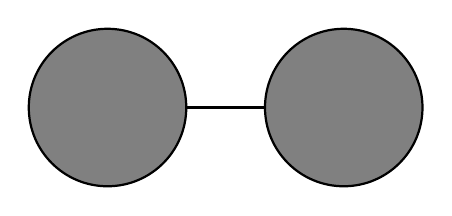
\begin{tikzpicture}
\draw[thick, fill=gray] (0,0) circle (1);
\draw[thick, fill=gray] (3,0) circle (1);
\draw[thick] (1,0) -- (2,0);
\end{tikzpicture}\end{image}
\begin{multipleChoice}
\choice[correct]{path-connected}
\choice{not path-connected}
\end{multipleChoice}

\item \begin{image}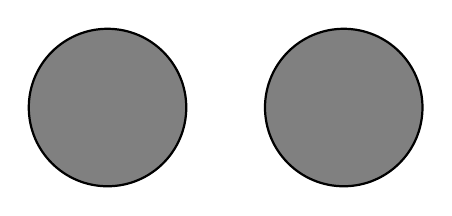
\begin{tikzpicture}
\draw[thick, fill=gray] (0,0) circle (1);
\draw[thick, fill=gray] (3,0) circle (1);
\end{tikzpicture}\end{image}
\begin{multipleChoice}
\choice{path-connected}
\choice[correct]{not path-connected}
\end{multipleChoice}

\end{enumerate}
\end{problem}

\section*{Simply Connected Sets}

The last topological concept we will cover is when a path-connected set is ``simply connected.'' Intuitively, this depends on whether or not the set has holes. Our definition for simply connected is a bit hand wavy, but this will serve our purpose just fine. It can be made rigorous using continuous maps. %(INCLUDE THIS SOMEWHERE?)

\begin{definition}
A path-connected set $X\subset\mathbb{R}^n$ is \emph{simply connected} if any closed path (i.e., loop) can be shrunk to a point, where the shrinking occurs entirely in $X$.
\end{definition}

%VIDEO

Note that a set needs to be path-connected in order to be considered simply connected.

\begin{problem}

For each of the following sets, determine whether or not they are simply connected.
\begin{enumerate}
\item $\mathbb{R}^2\setminus\{(0,0)\}$

\begin{image}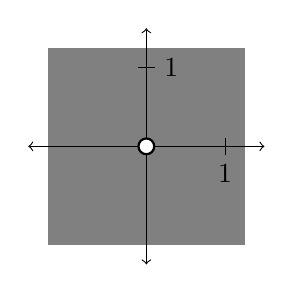
\begin{tikzpicture}
\fill[gray]
       (-1.25,-1.25) -- (-1.25,1.25) -- (1.25,1.25) -- (1.25, -1.25) -- cycle;

\draw[<->] (-1.5,0) -- (1.5,0);
\draw[<->] (0,-1.5) -- (0,1.5);
\draw[thick, fill=white] (0,0) circle (0.1);

\foreach \x in {1}
\draw[shift={(\x,0)},color=black] (0pt,3pt) -- (0pt,-3pt) node[below] 
{$\x$};

\foreach \y in {1}
\draw[shift={(0,\y)},color=black] (-3pt,0pt) -- (3pt,0pt) node[right] 
{$\y$};
\end{tikzpicture}\end{image}
\begin{multipleChoice}
\choice{simply connected}
\choice[correct]{not simply connected}
\end{multipleChoice}

\item $\mathbb{R}^2$

\begin{image}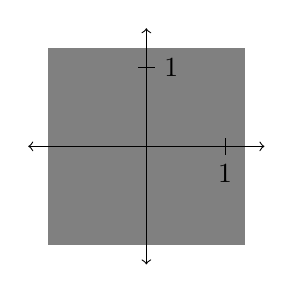
\begin{tikzpicture}
\fill[gray]
       (-1.25,-1.25) -- (-1.25,1.25) -- (1.25,1.25) -- (1.25, -1.25) -- cycle;

\draw[<->] (-1.5,0) -- (1.5,0);
\draw[<->] (0,-1.5) -- (0,1.5);

\foreach \x in {1}
\draw[shift={(\x,0)},color=black] (0pt,3pt) -- (0pt,-3pt) node[below] 
{$\x$};

\foreach \y in {1}
\draw[shift={(0,\y)},color=black] (-3pt,0pt) -- (3pt,0pt) node[right] 
{$\y$};
\end{tikzpicture}\end{image}
\begin{multipleChoice}
\choice[correct]{simply connected}
\choice{not simply connected}
\end{multipleChoice}

\item $\{(x,y,z)\,:\,x^2+y^2+z^2=1\}$

\begin{image}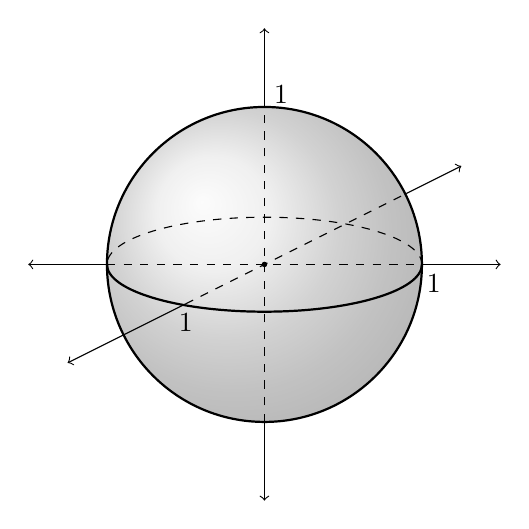
\begin{tikzpicture}
  \shade[ball color = gray!40, opacity = 0.4] (0,0) circle (2cm);
  \draw[thick] (0,0) circle (2cm);
  \draw[thick] (-2,0) arc (180:360:2 and 0.6);
  \draw[dashed] (2,0) arc (0:180:2 and 0.6);
  \fill[fill=black] (0,0) circle (1pt);
  
  \draw[<-] (-3, 0) -- (-2,0);
  \draw[dashed ] (-2,0 ) -- (2,0) node[below, xshift=1ex] 
{$1$};
  \draw[->] (2,0) -- (3,0);
  \draw[<-] (0, -3) -- (0,-2);
  \draw[dashed] (0,-2 ) -- (0,2) node[right, yshift = 1ex] 
{$1$};
  \draw[->] (0,2) -- (0,3);
  \draw[<-] (-2.5, -1.25) -- (-1,-0.5);
  \draw[dashed] (-1,-0.5) node[below] 
{$1$} -- (1.8, 0.9);
  \draw[->] (1.8, 0.9) -- (2.5, 1.25);
\end{tikzpicture}\end{image}

\begin{multipleChoice}
\choice[correct]{simply connected}
\choice{not simply connected}
\end{multipleChoice}

\item A torus (the surface of a donut)

\begin{image}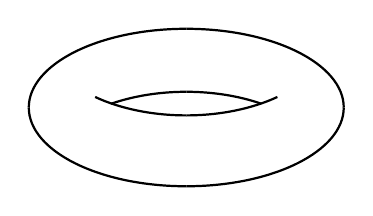
\begin{tikzpicture}
\draw[thick] (0,-1) arc (270:180:2 and 1);
\draw[thick] (0,-1) arc (270:360:2 and 1);
\draw[thick] (0,1) arc (90:0:2 and 1);
\draw[thick] (0,1) arc (90:180:2 and 1);
\draw[thick] (0,-.1) arc (270:230:1.8 and 1);
\draw[thick] (0,-.1) arc (270:310:1.8 and 1);
\draw[thick] (0,.2) arc (90:122:1.8 and 1);
\draw[thick] (0,.2) arc (90:58:1.8 and 1);
\end{tikzpicture}\end{image}
\begin{multipleChoice}
\choice{simply connected}
\choice[correct]{not simply connected}
\end{multipleChoice}

\end{enumerate}
\end{problem}






\end{document}